\chapter{Introduction} \label{intro}

Medical Software is a critical component of patient diagnosis and treatment. Medical software refers to computer programs, applications, or systems specifically designed for use within the healthcare and medical field. These software solutions are developed to assist healthcare professionals, researchers, administrators, and patients in various aspects of medical care, research, management, and education \cite{medical_software}. Our project focuses on medical software that could potentially influence a patients' well-being, particularly software that contributes to diagnosing issues related to the aorta. The aorta, a vital artery responsible for transporting blood from the heart to other bodily organs, holds immense significance. Any malfunction in its blood-carrying function could yield severe and potentially life-threatening consequences for the entire body's physiology. Specifically, we focus on the Aorta Geometry Reconstruction (AortaGeomRecon or AGR) software, which can build a 3-dimensional model of the aorta, to help the health professional diagnosing issues related to the aorta quickly and correctly.

Given the importance of medical software like AGR, we need a means to build confidence in the software. In this report, we explore the use of assurance cases. An assurance case can be thought of as a structured argument. The main purpose of an assurance case is to establish confidence and trust in the reliability and safety of a system by presenting a well-structured argument supported by evidence \cite{Weinstock_2013}. Assurance cases have been applied regularly in the medical device for approval in U.S. In Europe, the assurance cases are required in systems as diverse as flight control systems, nuclear reactor shutdown systems, and railroad signaling systems, which are all critical systems \cite{Weinstock_2013}. Previous work \cite{Nejad2017} \cite{scs_ac} investigating assurance cases for scientific computing software such as 3dfim+, a medical imaging software analyzing activity in the brain, has demonstrated the value of the technique in showing the software's correctness and reliability. The motivation of our project is to build on this previous work to more deeply investigate the necessary evidence. Specifically, we build an assurance case for AGR by adding more details on the evidence needed to support our correctness claims, thus building our confidence in AGR.

In this chapter, we first explain in details the contexts for the key concepts that will be discussed throughout the document, including what is organ segmentation, what is the aorta, listing the diseases that aorta segmentation could detect, and demonstrating an example of an assurance case by showing a simple example. Next, we will briefly discuss the methodology, especially how we achieve the objective of design, implementation of the software, and building confidence with the evidences in an assurance case. In the final section, we explain our report outline.

\section{Background} \label{bg}

In this section, we present the contexts of the key concepts within the scope of our work, including background information on the aorta (section \ref{aorta}), organ segmentation (section \ref{organ_seg}), and assurance cases (section \ref{ac}).

\subsection{Aorta}\label{aorta}
The aorta is the largest artery in the body. It carries blood from the heart to the circulatory system. It has a cane-liked shape made up of the ascending aorta, aortic arch and descending aorta. Figure~\ref{fig_aorta} shows the entire aorta, but the abdominal aorta is outside the scope of the current work. Our work focus on building the 3D geometry from the aortic root to descending aorta.

\begin{figure}[ht]
    \centering
    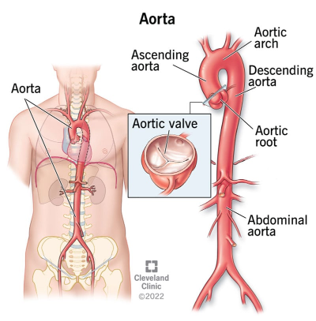
\includegraphics[width=0.35\textwidth]{figures/Intro/Aorta.png}
    \caption[Aorta]{Aorta \cite{Cleveland_Clinic_medical_professional_2021}}
    \label{fig_aorta}
\end{figure}

\subsection{Organ Segmentation}\label{organ_seg}
The definition of the organ boundary or organ segmentation is helpful for the orientation and identification of the regions of interest inside the organ during diagnostic or treatment procedures. Further, it allows the volume estimation of the organ, such as the aorta. A segmentation takes a medical image as input and outputs the portion of the image that corresponds to the organ of interest. Figure~\ref{fig_seg} demonstrates an example of abdominal organ segmentation.

\begin{figure}[ht]
    \centering
    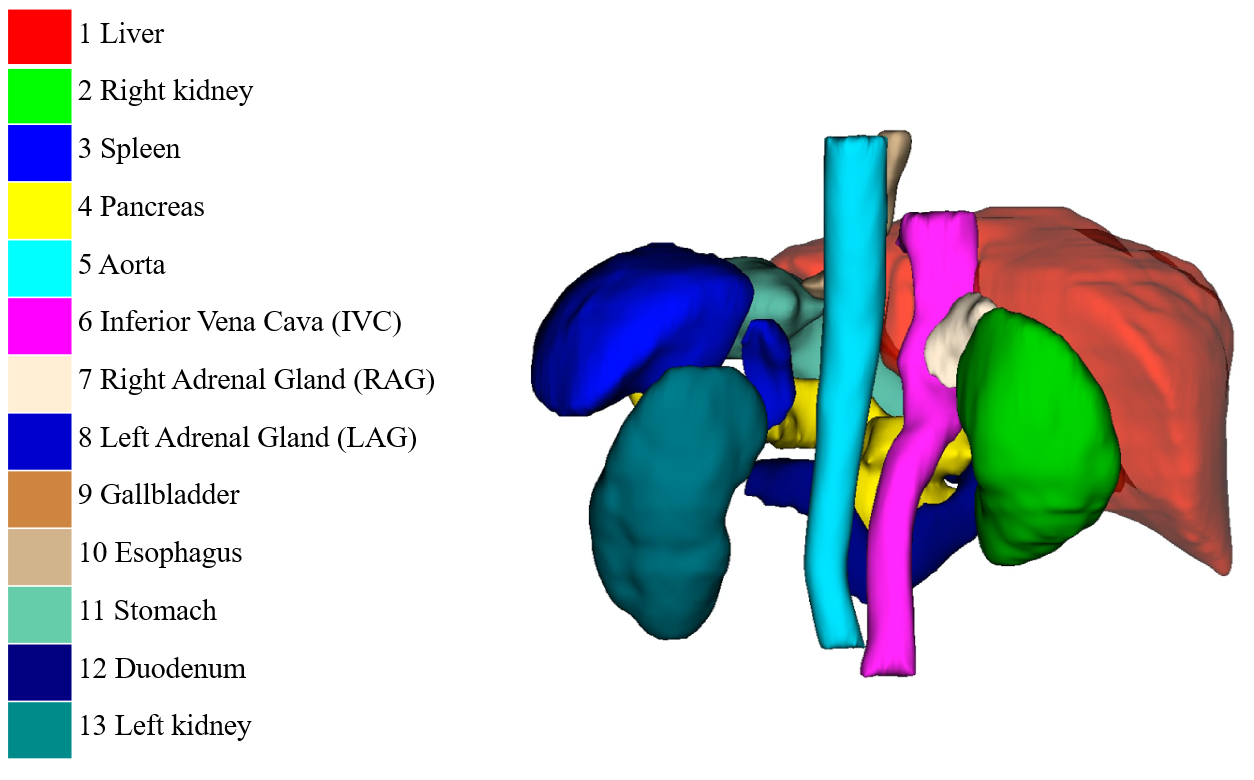
\includegraphics[width=0.7\textwidth]{figures/Intro/segmentation.png}
    \caption[Organ Segmentation]{Organ Segmentation \cite{Ma-2021-AbdomenCT-1K}}
    \label{fig_seg}
\end{figure}

Aorta segmentation in CT (Computerized Tomography) scans is important for diagnosing or treating:
\begin{itemize}
\item Coarctation of the aorta (narrowing of aorta)
\item Aortic aneurysm (bulge in the aorta)
\item Aortic calcification quantification
\item To guide the segmentation of other central vessels. 
\end{itemize} ~

\subsection{Assurance Case}\label{ac}
\begin{figure}[ht]
    \centering
    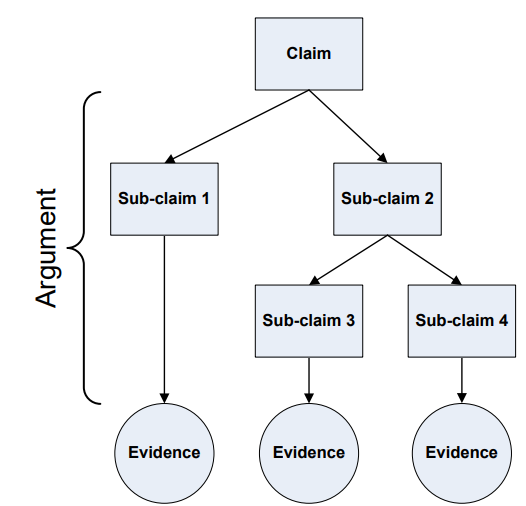
\includegraphics[width=0.45\textwidth]{figures/Intro/ac_diagram.png}
    \caption[Simple Assurance Case Diagram]{Simple Assurance Case Diagram \cite{doi:10.2514/6.2009-1921}}
    \label{fig_ac_diagram}
\end{figure}

An Assurance Case (AC) can be thought of as a structured argument. When building an AC, you're making a point that specific evidence backs up a particular statement. The fundamental structure is depicted in Figure \ref{fig_ac_diagram}. An AC essentially boils down to an organized collection of arguments, backed by a body of evidence, that helps validate the belief in a specific claim \cite{doi:10.2514/6.2009-1921}.

In a practical sense, creating an AC involves beginning with a main claim and then breaking it down into smaller claims through a step-by-step process. These smaller claims, at the most bottom, are supported by concrete evidence.


\section{Methodology} \label{methodology}
In this study, we present the outcomes of integrating AC throughout the development of medical software to reinforce the stakeholders' confidence in the software's capabilities. The software, known as AortaGeomRecon (AGR), represents a 3D Slicer \cite{Kikinis2014} extension module designed to semi-automatically construct a 3D model of the aorta using CT scans from a patient's chest. We started by gathering requirements for the AGR from a domain expert, drafted our requirements, and high-level design. We researched and worked on the implementation of the software, while building the infrastructure for continuous integration, version control, and project managment using GitHub. When we have a functional prototype, we delved into our assurance cases, encompassing chosen arguments and supporting evidence. AC functions as a method to provide assurance for a system by presenting arguments that substantiates claims about the system. These arguments are based on evidence related to the system's design, development, and tested behavior. By constructing the AC, we were able to follow the best practice including documentation review on the requirements and high-level design. Our goal was to finalize our documentation, and ensure the documentation's completeness and correctness. We have built user documentation to define all operational assumptions, and guide the user to use the valid inputs with a sequence of correct operations. Finally, our assurance case evidence consists of continuous integration tests, code review, and several algorithm reviews. This increased our confidence that the implementation of the software has strictly complied with the requirements and is  complete and correct.

\section{Thesis Outline} \label{TO}

The thesis is organized into three broad parts. In Chapter 2, we introduce our program \progname{} by mentioning the existing methods, the AGR's algorithm overview and step-by-step  workflow. We explain necessary terms and information to understand how the software functions. We also introduce the 3D Slicer \cite{Kikinis2014} extension module that the user interacts with to get the segmentation result with our algorithm. In Chapter 3, we present our AC, focusing on the evidence and including  some sections of our requirements, high-level design, detailed design, algorithm review, and a test case we developed for verifying and validating the correctness of AGR. In Chapter 4, future work is proposed and conclusions are drawn based on the developed requirements, segmentation algorithm, 3D Slicer module extension, and AC.